\documentclass[french]{hermes-journal}

\ria{2014}{28}{2-3}

\usepackage{textcomp}

%\usepackage{lmodern}
\usepackage{fontspec}%% load unicode fonts for xelatex

%\DeclareUnicodeCharacter{00A0}{~}
%\DeclareUnicodeCharacter{00DF}{\ss}
%\DeclareUnicodeCharacter{00E4}{\"a}

% pagination
\firstpagenumber{1}

\newcommand*{\lpath}{./}
%\usepackage[cmex10]{amsmath, mathtools}
%\usepackage{amsmath,amssymb,amsbsy,amsfonts,amsthm}
%\usepackage[ruled,vlined]{algorithm2e}
\usepackage{amsmath,amssymb,amsbsy,amsfonts}
\usepackage{mathtools}
\usepackage{booktabs}
\usepackage{multirow}
\usepackage{bm}
\usepackage{enumerate}
\usepackage{url}
\usepackage{fancyvrb}
\usepackage{yfonts}
\usepackage{wrapfig}
\usepackage{subfigure}
\usepackage{tikz}
\usetikzlibrary{bayesnet}
\newcommand{\tikzmark}[1]{\tikz[overlay,remember picture] \node (#1) {};}
\usepackage{calc}%    For the \widthof macro
\usepackage{xparse}%  For \NewDocumentCommand
\usepackage{adjustbox}


%% Variable de compilation
\newif\ifbeamer
\beamerfalse
\newcommand{\beamer}[2]{\ifbeamer #1 \else #2 \fi}
%%%

%\usepackage[latin1]{inputenc}
\usepackage[utf8]{inputenc} % manage utf8 encodage 
%\usepackage[english]{babel} % for french document ! dirty enumerate style,+ bad change rectangle colors for section linking.
\usepackage{fancyhdr} % for heading
\usepackage{listings}
\usepackage[colorlinks=true, urlcolor=blue]{hyperref} % url, link
\usepackage{graphicx}
\usepackage{geometry}

%\usepackage[cmex10]{amsmath, mathtools}
\usepackage{amsmath,amssymb,amsbsy,amsfonts,amsthm}
\usepackage{multirow}
\usepackage{bm}
\usepackage{enumerate}
\usepackage{url}
\usepackage[ruled,vlined]{algorithm2e}
\usepackage{fancyvrb}
\usepackage{yfonts}

\usepackage{wrapfig}
\usepackage{tikz}
    %\input{../tikz.conf}
    
\usetikzlibrary{bayesnet}
    
%%%%%%%%%%% Box 
\usepackage{calc}%    For the \widthof macro
\usepackage{xparse}%  For \NewDocumentCommand
\newcommand{\tikzmark}[1]{\tikz[overlay,remember picture] \node (#1) {};}

%%%%%%%%%% Math
\renewcommand{\text}{\textnormal}
\newcommand{\pr}{\mathbf{p}}
\newcommand{\E}{\mathbb{E}}
\newcommand{\divkk}{\mathbb{K}}
\newcommand{\entropy}{\mathbb{H}}
\newcommand{\gem}{\mathrm{GEM}}
\newcommand{\Mult}{\mathrm{Mult}}
\newcommand{\DP}{\mathrm{DP}}
\newcommand{\IBP}{\mathrm{IBP}}
\newcommand{\M}{\mathcal{M}}
\newcommand{\V}{\mathcal{V}}
\newcommand{\N}{\mathcal{N}}
    
\makeatletter
\NewDocumentCommand{\DrawBox}{s O{}}{%
    \tikz[overlay,remember picture]{
    	\IfBooleanTF{#1}{%
    		\coordinate (RightPoint) at ($(left |- right)+(\linewidth-\labelsep-\labelwidth,0.0)$);
    	}{%
    	\coordinate (RightPoint) at (right.east);
    }%
    \draw[red,#2]
    ($(left)+(-0.2em,0.9em)$) rectangle
    ($(RightPoint)+(0.2em,-0.3em)$);}
}

\NewDocumentCommand{\DrawBoxWide}{s O{}}{%
	\tikz[overlay,remember picture]{
		\IfBooleanTF{#1}{%
			\coordinate (RightPoint) at ($(left |- right)+(\linewidth-\labelsep-\labelwidth,0.0)$);
		}{%
		\coordinate (RightPoint) at (right.east);
	}%
	\draw[red,#2]
	($(left)+(-\labelwidth,0.9em)$) rectangle
	($(RightPoint)+(0.2em,-0.3em)$);}
}
\makeatother
%%%%% ! Box

\geometry{
      a4paper,
	    body={160mm,260mm},
	    left=25mm,top=20mm,
	    headheight=4mm,headsep=8mm,
        footskip=10mm,
        }
                                              

%%%%%%%%%%%%%%%%%%%%%%%%%%%%%%%%%%%%%%%%%%%%%%%%%%%%%%%%%%%%%%%%%%%%%%%%%%%%%%%%%%%%%%%%%%%%%%%%%%%%%%
%%%%% => Internal
%%%%%%%%%%%%%%%%%%%%%%%%%%%%%%%%%%%%%%%%%%%%%%%%%%%%%%%%%%%%%%%%%%%%%%%%%%%%%%%%%%%%%%%%%%%%%%%%%%%%%%

% itemize item def
%% \begin{itemize}\itemsep2pt % example space betwew item
%\renewcommand{\FrenchLabelItem}{\textbullet}
\renewcommand{\labelitemi}{$\bullet$}
\renewcommand{\labelitemii}{$\cdot$}
\renewcommand{\labelitemiii}{$\diamond$}
\renewcommand{\labelitemiv}{$\ast$}

% equation reference
\renewcommand{\theequation}{\thesection.\arabic{equation}}

%%%%%%%%%%%%%%%%%%%%%%%%%%%%%%%%%%%%%%%%%%%%%%%%%%%%%%%%%%%%%%%%%%%%%%%%%%%%%%%%%%%%%%%%%%%%%%%%%%%%%%
%%%%% => Alias
%%%%%%%%%%%%%%%%%%%%%%%%%%%%%%%%%%%%%%%%%%%%%%%%%%%%%%%%%%%%%%%%%%%%%%%%%%%%%%%%%%%%%%%%%%%%%%%%%%%%%%

% write code
\lstnewenvironment{C}[1]
{\lstset{language=C,
      frame=tBRl,
      basicstyle=\scriptsize,stringstyle=\emph,showstringspaces=false,
      numbers=left,numberstyle=\tiny,
      breaklines=true, columns=flexible, title={#1}}
}{}
      
%%%%%%%%%%%%%%%%%%%%%%%%%%%%%%%%%%%%%%%%%%%%%%%%%%%%%%%%%%%%%%%%%%%%%%%%%%%%%%%%%%%%%%%%%%%%%%%%%%%%%%
%%%%% => Preambles Pages
%%%%%%%%%%%%%%%%%%%%%%%%%%%%%%%%%%%%%%%%%%%%%%%%%%%%%%%%%%%%%%%%%%%%%%%%%%%%%%%%%%%%%%%%%%%%%%%%%%%%%%

\pagestyle{fancy}
\fancyhf{} % remove default headers
\fancyfoot[C]{\thepage}
\renewcommand{\footrulewidth}{0.3pt}
\renewcommand{\headrulewidth}{0.3pt}

%%%%%%%%%% Math
\renewcommand{\text}{\textnormal}
\newcommand{\ilfm}{\texttt{ILFM}}
\newcommand{\immsb}{\texttt{IMMSB}}
\newcommand{\mmm}{\texttt{Mixed-Membership}~}
\newcommand{\pr}{p}
\newcommand{\p}{p}
\newcommand{\E}{\mathbb{E}}
\newcommand{\divkk}{\mathbb{K}}
\newcommand{\entropy}{\mathbb{H}}
\newcommand{\gem}{\mathrm{GEM}}
\newcommand{\Mult}{\mathrm{Mult}}
\newcommand{\DP}{\mathrm{DP}}
\newcommand{\IBP}{\mathrm{IBP}}
\newcommand{\M}{\mathcal{M}}
\newcommand{\V}{\mathcal{V}}
\newcommand{\N}{\mathcal{N}}
\newcommand{\mat}[1]{\bm{#1}}
\newcommand{\unit}{1\!\!1}

%\newtheorem{definition}{Definition}[section]
%\newtheorem{proposition}{Proposition}[section]
%\newtheorem{theorem}{Theorem}[section]
%\newtheorem{corollary}{Corollary}[section]


%\title[short header title]{title}
\title[]{Une Etude des Modèles Mixed-Membership pour la Prédiction de Liens dans les Réseaux Sociaux}

\author[1]{Adrien}{Dulac}
%\author[2]{first name 2}{last name 2}
%
%% addresses are automatically numbered
%\address{...\\...\\
%         ..., country}
%        {e-mail 1}
%\address{...\\...\\
%         ..., country}
%        {e-mail 1}

%\author{\IEEEauthorblockN{Adrien Dulac\IEEEauthorrefmark{1}, Eric Gaussier\IEEEauthorrefmark{1} and Christine Largeron \IEEEauthorrefmark{2}}\\
%\IEEEauthorblockA{\IEEEauthorrefmark{1}
%Univ. Grenoble Alpes, CNRS, Grenoble INP, LIG - F-38000 Grenoble\\
%Email: \{adrien.dulac, eric.gaussier\}@imag.fr}
%\IEEEauthorblockA{\IEEEauthorrefmark{2}
%Univ Lyon, UJM-Saint-Etienne, CNRS, Institut d'Optique Graduate School,\\
%Laboratoire Hubert Curien UMR 5516, F-42023, SAINT-ETIENNE, France\\ 
%Email: christine.largeron@univ-st-etienne.fr}}

\abstract{We assess here whether standard stochastic mixed membership models are adapted for link prediction in social networks by studying how they handle homophily and preferential attachment. To study these properties, we first introduce formal definitions of these phenomena; we then study how stochastic mixed membership models relate to these definitions. Our theoretical analysis reveals that standard stochastic mixed membership models comply with homophily with the similarity that underlies them. For preferential attachment, the situation is more contrasted: if these models do not comply with global preferential attachment, their compliance to local preferential attachment depends on whether the memberships to latent factors are hard or soft, and in the latter case on whether the underlying latent factor distribution is bursty or not. We illustrate these elements on synthetic and real networks by using the generative properties of Bayesian model.}

\resume{Nous évaluons dans ce papier si la classe de modèle, dit mixed-membership, est adapté pour la prédiction de liens dans les réseaux sociaux en étudiant leurs comportements vis-à-vis de l'homophilie et de l'attachement préférentiel. Pour étudier ces propriétés, nous introduisons les définitions de ces phénomènes, après quoi nous étudirons comment ces modèles sont reliés à ces définitions. Notre étude théorique révèle que les modèles mixed-membership satisfont l'homophilie avec la similarité naturelle qui les sous-tend. Pour l'attachement préférentiel la situation est plus contrasté: ces modèles ne satisfont pas l'attachement préférentiel global. En revanche, le respect de l'attachement préférentiel local est possible selon que l'appartenance au classes latentes soit strict ou léger. Et dans ce dernier cas si la distribution sur les classes latentes est bursty ou pas. Nous illustrons ces éléments sur des réseaux réels et synthétiques grâce aux propriétés génératives des modèles Bayésiens.}

\keywords{Hierachical baysian Models, Random Graph, Machine Learning, Social Networks}

\motscles{Modèle Bayesian Hérarchique, Graphe aléatoire, Apprentissage Automatique, Réseaux Sociaux}


%
%
%
%  Is  better abstract
%
%
%\significancestatement{We introduce formal definitions of the compliance of probabilistic link prediction models to homophily and preferential attachment in social networks, and show that standard stochastic mixed membership models comply with homophily with the similarity that underlies them. For preferential attachment, the situation is more contrasted: if these models do not comply with global preferential attachment, their compliance to local preferential attachment depends on whether the memberships to latent factors are hard or soft, and in the latter case on whether the underlying latent factor distribution is bursty or not.}


\begin{document}

\maketitle

\newpage

\section{Introduction}

\label{sec:intro}

Plusieurs modèles de prédictions de liens puissants ont été proposés dans la littérature pour apporter une solution au problème dit de \textit{prédiction de liens} consistant à prédire la probabilité d'une relation entre deux noeud quelconque dans un réseaux social \cite{LibenNowell07, HassanZaki11}.
Parmi ces modèles, la classe des modèles \mmm a reçu une attention particulière due à leurs capacité à faire émerger la structure d'un réseaux et d'inférer des liens non observés.
Deux instances principale de cette classe ont été proposés et étudiés  dans la littérature : le modèle à composition mixte de bloc (MMSB) \cite{MMSB} et son extension non-paramétrique \cite{iMMSB, fan2015dynamic} d'un coté et le modèle à attributs latents (ILFM) \cite{BMF} et son extension non-paramétrique \cite{ILFRM} de l'autre. 


Les modèles probabilistes, tel que ceux considérés sont usuellement évalué empiriquement. Néanmoins, les réseaux sociaux réels exhibent des propriétés générales qui permettent de les caractériser Dans ce papier, nous traitons deux propriétés importantes, \textit{l'homophilie} et \textit{l'attachement préférentielle} \cite{Newman2010, Barabasi2003}. Nous étudions dans quelle mesures les modèles de prédictions de liens, de la classe mentionné, se conforment à elles. 

L'homophilie est une propriété qui correspond à l'idée que la probabilité que deux nœuds du réseaux soient liés augmente avec leurs similarités et communément suggérer par la locution \emph{"qui se ressemble s'assemble"}.

L'attachement préférentielle est une propriété d'avantage "topologique" dans le sens ou les ne dépend que du nombre de connections présentes dans le réseaux. Elle signifie que la probabilité de créer un liens avec un autre noeud dépend du nombre de liens de ce dernier (son degré). Cette propriété est d'une certaine façon, l'image de l'aphorisme populaire \emph{"On ne prête qu'aux riches"}. En théorie des graphes l'attachement préférentiel est évoqué pour expliquer l'émergence de graphes dit "scale-free" qui sont caractérisé par une distribution des degrés en loi de puissance.

L'intérêt de ces propriétés dans l'analyse des réseaux sociaux a été largement mise en avant pour la modélisation de réseaux et l'amélioration des taches de prédictions de liens comme de détection de communauté.


\section{Related Work}

On doit mettre ue section related work ? ou on plus de ref dans l'intro suffisant ?

\section{Modèles de prédictions de liens stochastique}

Les modèles \mmm sont des modèles génératifs basé sur des facteurs latent (aussi appelé classe latentes ou caractéristiques latentes) qui représente les propriétés, a priori, des noeuds du graphe $G=(V,E)$ associé au réseaux social (chaque noeud représente un individu); Nous notons la matrice d'adjacence associé $Y=(y_{ij})_{i,j\in V}$ et ou $y_{ij}=1$ si un liens est observé entre $i$ et $j$ et $y_{ij}=0$ si un non-lien est observé. Nous dénotons $N$ le nombre de noeud du graphe ($N=|V|$). Les modèles \mmm sont caractériser par le fait qu'un noeud peut appartenir à plusieurs facteurs latents. Par exemple, cela peut permet de modéliser le fait qu'un individu puisse appartenir à plusieurs communautés \footnote{Comme mentionné dans \cite{goldenberg2010survey} }. L'appartenance d'un noeud $i$ est encodé dans son facteur latent par un vecteur $\mat{f}_i$ de dimension finie $K$ dans les version standard des modèles, et de dimension potentiellement infinie dans les versions non-paramétriques, et cette dimension devient un paramètre du modèle. La collection des vecteurs $\mat{f}_{i}$ ($1 \le i \le N$) constitue la matrice de caractéristique latentes $\mat{F}$. De plus, une matrice de poids $\mat{\Phi}$ est utilisé pour encoder les corrélations entre les caractéristiques latentes. Comme nous travaillons sur des réseaux binaire, les observations (liens) sont ont pour vraisemblance un distribution de Bernoulli.

Les modèles de la classe des \mmm diffèrent dans la manière dont les matrices $\mat{F}$ et $\mat{\Phi}$ sont générées Afin de rester dans un cadre le plus général possible, nous considérons ici les versions non-paramétriques du modèles de caractéristique latentes \cite{ILFRM}, dénoté \ilfm, et du modèle de composition mixte bloc  \cite{iMMSB,fan2015dynamic}, dénoté \immsb. Cela conduit à un nombre de facteur latent dynamique qui permet à la dimension du modèles de s'adapter à la compléxité des données. En pratique, cela est réalisé par l'utilisation de prior non-paramétrique, le processus de Dirichlet Hiérarchique (HDP) pour \immsb\ et le processus du Buffet Indien (IBP) for \ilfm.~\\

Concernant \ilfm, chaque noeud du réseau est représenté par un vecteur de caractéristique binaire. La probabilité de créer un lien entre deux noeuds dépend alors uniquement de la matrice de caractéristique latente et de la matrice  de poids, ou chaque entrée est généré par une distribution normale. La matrice de caractéristique est généré via un IBP, conduisant à un nombre de caractéristique théoriquement infini, bien que pour un nombre fini d'observation (de liens), seulement un nombre finis de caractéristiques sont active). Le processus génératif se résume ainsi :
\begin{enumerate}
\item Generation d'une matrice de caractéristiques $\mat{F}_{N \times \infty}$ : $\mat{F} \sim \IBP(\alpha)$
\item Generation d'une matrice de poids : $\mat{\phi}_{mn} \sim N(0, \sigma_w), \, m,n \in \mathbb{N}^{+*}$
\item Generation d'un lien (ou non lien) pour chaque couple de noeud $(i,j)$ : 
\begin{equation*}
y_{ij} \sim \mathrm{Bern}(\sigma(\mat{f}_{i} \mat{\Phi} \mat{f}_{j}^\top))
\label{eq:link-ilfm}
\end{equation*}
\end{enumerate}
%

Ou $\top$ représente la transposé et $\sigma$ la fonction sigmoïde permettant de passer d'un ensemble $[-\infty, +\infty]$ vers un ensemble de probabilité $[0,1]$.  $\mat{f}_{i}$ dénotes la i-ème ligne de la matrice $F$ comme le vecteur de caractéristique latent du noeud $i$. Finalement, ce modèle définit deux hyper-paramètres, l'un étant le paramètre de concentration $\alpha$ de IPB, et l'autre pour la variance de la distribution normale des poids $\sigma_w$. Dans le cas d'un réseau dirigé, les matrices $\mat{Y}$ et $\mat{\Phi}$ sont symétriques et uniquement leur partie diagonal supérieur (ou inférieur) sont générés. ~\\


Le modèle \immsb quand à lui, génère les distributions d'appartenance aux des classe latentes à partir d'un processus (hiérarchique) de Dirichlet. Après quoi, une appartenance de classe latentes par noeud est tirée pour chaque couples de noeud. Finalement, la probabilité de connecter deux liens est tiré en fonction du poids encodant la corrélation entre ces deux classes, se résumant au processus génératif suivant :
\begin{enumerate}
\item Generation des distributions des classes d'appartenances $\mat{F}_{N \times \infty}$:
   \begin{align}
       \bm{\beta} &\sim \gem(\gamma) \nonumber \\
    \mat{f}_i &\sim \DP(\alpha_0, \beta) \quad\text{ for }  i \in \{1, .., N\} \nonumber
   \end{align}  Ou $\gem$ dénote le processus Stick-Breaking Process qui est une distribution sur la ligne réel et $\DP$ un processus de Dirichlet \cite{HDP}.
\item Generation de la matrice de poids depuis une distribution Beta :\\
\[ \phi_{mn} \sim \mathrm{Beta}(\lambda_0,\lambda_1), \, m,n \in \mathbb{N}^{+} \]
\item Génération de classes d'appartenances pour la dyade pour chaque couple de noeud $(i,j)$ tirés d'un loi multinomiale et genération d'un lien (ou non-lien) : 
   \begin{align}
       z_{i \rightarrow j} \sim&\ \mbox{Cat}(\mat{f}_i) \quad z_{i \leftarrow j} \sim \mbox{Cat}(\mat{f}_j) \nonumber \\
       y_{ij} &\sim \mathrm{Bern}(\phi_{z_{i \rightarrow j}z_{i \leftarrow j}}) \nonumber
    \label{eq:link-immsb}
   \end{align}
\end{enumerate}


Ce modèle contient quatre hyper-paramètres, $(\gamma, \alpha_0)$ pour le HDP et $(\lambda_0, \lambda_1)$ pour la distribution des poids. La remarque s'applique le modèle précèdent concernant les réseaux dirigés.

Dans l'usage classique des modèles décrits pour la prédiction de liens, des observations (liens) sont disponibles et sont utilisés pour estimer  $\mat{F}$ et $\mat{\Phi}$, a partir desquels de nouveaux liens peuvent être prédit. Dans la suite de ce papier, nous dénoterons par $\mat{\hat{F}}$ et $\mat{\hat{\Phi}}$ les estimations (ie paramètres inférés) de $\mat{F}$ et $\mat{\Phi}$, qui peuvent être obtenue à partir d'algorithme inférence approximé tel que le (collapsed) Gibbs sampling et Metropolis-Hastings ou encore à l'aide d'inférence variationnelle Nous ne les détaillons pas ici et renvoyons le lecteur intéressé à \cite{ILFRM,IBP,HDP,fan2015dynamic}.

Nous dénoterons aussi $\mathcal{M}_e$ la version des deux modèles \ilfm\ and \immsb\ dans lesquels $\mat{F}$ and $\mat{\Phi}$ sont assumés connus et fixé à $\mat{\hat{F}}$ et  $\mat{\hat{\Phi}}$.

Nous nous tournons maintenant sur l'analyse de ces propriété par les modèles \mmm, à savoir, a partir des paramètres appris $\mat{\hat{F}}$ and $\mat{\hat{\Phi}}$.


\section{Homophilie: \emph{"Birds of a feather flock together"}}
\label{sec:homophily}

L'homophilie réfère à la tendance aux individus de se connecter à d'autres similaires  \cite{mcpherson2001birds,lazarsfeld1954friendship}. La similarité considéré est souvent considéré de manière inhérentes aux individus et peut représenter leur statut, leurs préférences ou intérêts Une notion proche est celle d'\emph{assortativité}, qui est plus général et s'applique à tout type de réseaux, pas seulement sociaux, et souvent utilise le degré en guise de similarité.


Une définition de l'homophilie à été proposé par \cite{la2010randomization}. Cependant, cette définitions ne s'appuie que sur une seul caractéristique (ie l'age ou le genre), et ne peut donc psa s'appliquer dans le cadre de modèles \mmm.

Nous introduisons donc la définitions d'homophile comme suit : 
\begin{definition}[Homophilie] \label{def:homophily}
    Suppose $\mathcal{M}_e$ est un modèle de prédiction de liens et $s$ une mesure de similarité entre noeuds. Nous disons que $\mathcal{M}_e$ est homophilique avec une similarité $s$ ssi, $\forall (i,j,i',j') \in V^4$:
\begin{equation}
s(i,j) > s(i',j')  \implies \pr(y_{ij}=1 \mid \mathcal{M}_e) > \pr(y_{i'j'}=1  \mid \mathcal{M}_e) \nonumber
\end{equation}

\end{definition}

\noindent Cette définition capture directement l'effet \emph{"plus deux noeuds sont similaires, plus ils ont une chance se connecter"}. 

Différentes similarités peuvent être considéré, tant qu'elles sont basé sur la mesures des propriété des noeuds considérés. Dans les modèles \mmm, ces propriété ne sont pas directement observé, et sont encodé dans les caractéristique latentes. D'après les paramètres des modèles, nous définition la notions de similarité naturelle comme étant $s_n(i,j) = \mat{\hat{f}}_{i} \mat{\hat{\Phi}} \mat{\hat{f}}_j^\top$.


On peut voir que les deux \ilfm\ and \immsb\, dans le contexte $\mathcal{M}_e$ sont homophiliques avec le respect de $s_n$. En effet, $\pr(y_{ij}=1 \mid \mathcal{M}_e)$ augmente avec $s_n$  pour  \ilfm\ comme la fonction sigmoïde est strictement croissante (Eq.~\ref{eq:ilfm}). De plus, en marginalisant sur les paramètres $z$ dans \immsb\ conduit à :
\begin{align}
    \pr(y_{ij} =1 \mid \mathcal{M}_e) & = \sum_{k,k'} \pr(y_{ij}=1|\mathcal{M}_e) \pr(z_{i \rightarrow j}=k | \mathcal{M}_e) \pr(z_{i \leftarrow j}=k' | \mathcal{M}_e) \nonumber \\
& = \sum_{k,k'} \hat{\phi}_{k,k'} \hat{f}_{ik} \hat{f}_{jk'} = \mat{\hat{f}}_{i} \mat{\hat{\Phi}} \mat{\hat{f}}_j^\top \nonumber
\end{align}


Nous définissons une seconde similarité uniquement dépendantes des caractéristiques latentes, ou ma matrice des poids est abandonné définie par $s_l(i,j) = \mat{\hat{f}}_{i} \mat{\hat{f}}_j^\top$. Avec cette similarité, ni \ilfm~ ou \immsb~ sont homophilique. En effet, assumons que $\mat{\hat{\Phi}}$ est presque nul sur la diagonal, est strictement positive ailleurs (ce qui est possible pour les deux modèles). Pour \immsb~ on a :
\begin{align*} 
\pr(y_{ij}=1 \mid \M_e) & = \sum_{k' \neq k} \hat{f}_{ik} \hat{\phi}_{kk'} \hat{f}_{jk'}
\end{align*}


Ici $\hat{\phi}_{kk} = 0$.  Considérons maintenant le paramétrage suivant: $\mat{\hat{f}}_i=\mat{\hat{f}}_j=(0,1,0)$ et $\mat{\hat{f}}_{i'}=(0.5,0,0.5)$ et $\mat{\hat{f}}_{j'}=(0,1,0)$. Alors, $s_l(i,j)=1$ et $s_l(i',j')=0$. Ainsi $\pr(y_{ij}=1 \mid \M_e) = 0$ alors que $\pr(y_{i'j'}=1 \mid \M_e) > 0$. Donc \immsb~ n'est pas homophilique avec $s_l$. De la mème manière, en remplaçant $\mat{\hat{f}}_{i'}=(0.5,0,0. 5)$ par $\mat{\hat{f}}_{i'}=(1,0,1)$, on voit que \ilfm~ n'est pas homophilique non plus avec $s_l$.

Cela montre que, pour qu'un modèle soir homophilique, il devrait être désigné en fonction de la similarité considéré pour la proximité entre individus. \ilfm et \immsb sont désigné sur la base de la similarité naturelle qui constitue le paramètre de la distribution de Bernoulli sur les liens, il est donc trivialement vrai que les modèles soit homophillique avec $s_n$. Il est néanmoins possible de rendre les modèles homophilique avec $s_l$ en adaptant le prior sur la matrice $\mat{\Phi}$; par exemple, une matrice de poids diagonal avec des poids constants conduiras à des modèles homophilique. Dans ce cas, les caractéristiques latentes peuvent être interprété comme des communautés. C'est ce qui est réalisé dans les travaux de \cite{AMMSB} afin de détecter des communauté recouvrante dans des réseaux sociaux.

\section{Attachement Préférentiel: \emph{"The rich get richer"}}
\label{sec:burstiness}


L'attachement préférentiel est un propriété d'un réseaux selon laquelle la probabilité qu'un noeud créer un liens avec un autre augmente avec le nombre de liens déja établi de ce dernier (son degré). Cette propriété est lié un phénomène plus général appelé \textit{burstiness} \footnote{A.L. Barab\'asi, par exemple, utilise ce terme\textit{attachement préférentiel} in \cite{barabasi1999emergence}, et \textit{burstiness} dans \cite{barabasi_burst}.} qui décrit le fait que certains évènements apparaissent en "rafale", c'est à dire qu'une fois qu'il apparaisse ils ont plus de chance d'apparaître encore. La burstiness a été étudié dans différents domaine, notamment en traitement automatique de langage et recherche d'information afin de caractériser l'occurrence des mots \cite{church1995poisson}. Des définitions simple du burstiness ont été proposé \cite{clinchant2008bnb,clinchant2010information}, pour les distribution continue et discrète, qui capturent le fait que la probabilité de nouvelles occurrences d'un évènement augmente avec le nombre d'occurrence de cet évènement. Nous adaptons ici ces définitions pour l'attachement préférentiel dans les réseaux. De plus, le phénomène peut apparaître a différent niveaux du réseaux : (a) l'attachement préférentiel global traite du degré sur l'ensemble des noeud et (b) l'attachement préférentiel local traite le degré au sein d'un classe (latentes) : 


\begin{definition}[Attachement préférentiel]
Soit $i$ un noeud dans un réseau social et soit $d_i$ son degré.
\begin{description}
    \item[(1)] \emph{Attachement préférentiel global}: on dit que le modèle de prédiction de liens $\mathcal{M}_e$ satisfait l'attachement préférentiel global ssi, pour chaque noeud $i$, $\pr(d_i \ge n+1 \mid d_i \ge n, \mathcal{M}_e)$ augmente avec $n n \in {0, N-1}$;
 \item[(2)] \emph{Attachement préférentiel local}: On dit que le modèle de prédiction de liens  $\mathcal{M}_e$ satisfait l'attachement préférentiel local ssi, pour chaque noeud $i$ muni de son degré local $d_{i,k}$ étant son degré au sein de la classe $k$, $\forall \epsilon \in [0,1], \, \pr(d_{i,k} \ge x+\epsilon \mid d_{i,k} \ge x, \mathcal{M}_e)$  augment avec $x \in [0,N-1]$. De plus , $d_{i,k}$ est défini comme l'espérance du degré de $i$ au sein de la classe $k$.
\end{description}
\label{def:burst-soc-net}
\end{definition}


Ces définitions traduisent directement le fait que plus un noeud à de connections plus il aura de chance d'en avoir de nouvelles. La différence entre le cas global et local est que le degré est généralement inconnue dans le cas local, et est ici estimé par son espérance

Pour l'attachement préférentiel global, le degré $d_i$ corresponds au nombre liens du noeud $i$. En exploitant le fait que les observations sont indépendantes étant donné $\mat{\hat{F}}$ et $\mat{\hat{\Phi}}$, nous avons:


\begin{align}
\pr(d_{i} \ge n+1 \mid d_{i} \ge n, \mathcal{M}_e) = 1 - \prod_{j \notin \mathcal{V}(i)} p(y_{ij} = 0 \mid d_{i} \ge n, \mathcal{M}_e) \nonumber \\
= 1 - \prod_{j \notin \mathcal{V}(i)} (1 - p(y_{ij} = 1 \mid d_{i} \ge n, \mathcal{M}_e)) \nonumber
\end{align}

Ou $\mathcal{V}(i)$ dénote l'ensemble des noeuds connecté à $i$. Soit $c=\min_{j \in V}  (1-p(y_{ij} = 1 \mid d_{i} \ge n, \mathcal{M}_e))$. Nous avons:

\[
0 \le \pr(d_{i} \ge n+1 \mid d_{i} \ge n, \mathcal{M}_e) \le (1 - c^{N-n}) \xrightarrow[n \rightarrow N]{} 0
\]

Cela montre que $\pr(d_{i} \ge n+1 \mid d_{i} \ge n, \mathcal{M}_e)$ n'augmente pas avec $n$. Nous avons donc la propriété suivante:

\begin{proposition}[]
\label{pref-attch-glob}
\ilfm\ et \immsb\ ne satisfont pas l'attachement préférentiel global.
\end{proposition}

Concernant l'attachement préférentiel local, la situation est plus complexe :

\begin{proposition}[]
\label{pref-attch-loc}
\immsb\ satisfait l'attachement préférentiel local alors que \ilfm\ ne le satisfait pas.
\end{proposition}

\noindent \textbf{Preuve (esquisse)} Soit $y_{ij,k}$ une variable aléatoire binaire qui est à 1 si le noeud $i$ et $j$ ont une connections au travers de classe latente $k$ et 0 autrement.
Alors $d_{i,k} = \sum_{j \in V} \pr(y_{ij,k} =1 | \mathcal{M}_e)$.
Pour \immsb, cela conduit à $d_{i,k} = \sum_{j \in V} \hat{f}_{ik} \hat{\Phi}_{kk} \hat{f}_{jk} = \hat{f}_{ik} \sum_{j \in V} \hat{\Phi}_{kk} \hat{f}_{jk}$.
L'effet de renforcement positive du processus de Dirichlet \cite{HDP} à la base de \immsb\ corresponds à phénomène bursty et se traduit, pour chaque $i$ et $k$, comme: $\pr(\hat{f}_{ik} \ge x'+\epsilon' \mid \hat{f}_{ik} \ge x',\mathcal{M}_e)$ augmente avec  $x'$ (pour tout $\epsilon'$ et $x'$ choisit en fonction du domaine définition de  $\hat{f}_{ik}$).
En posant $x=x'(\sum_{j\in V} \hat{\Phi}_{kk} \hat{f}_{jk})$ et $\epsilon = \epsilon'(\sum_{j\in V} \hat{\Phi}_{kk} \hat{f}_{jk})$ et en exploitant le fait que $\sum_{j\in V} \hat{\Phi}_{kk} \hat{f}_{jk}$ est positif et indépendant de $i$ conduit à : $\pr(d_{i,k} \ge x+\epsilon \mid d_{i,k} \ge x, \mathcal{M}_e)$ augmente avec $x$, ce qui prouve que \immsb\ satisfait l'attachement préférentiel local.

Pour \ilfm, posons $C_{i,k} = |\{j \in V, \hat{f}_{jk} = \hat{f}_{ik} = 1\}|$. Comme la matrice de caractéristique est binaire, nous avons: 

\[ 
d_{i,k} = \sum_{j\in V} \sigma(\hat{f}_{ik} \hat{\Phi}_{kk} \hat{f}_{jk}) =  C_{i,k} (\sigma(\hat{\Phi}_{kk})-0.5) + \frac{N}{2}
\]

Comme $\hat{f}_{ik}$  est binaire, il n'y a pas d'effet de  renforcement positif: $C_{i,k}$n'augmente pas si $\hat{f}_{ik}=1$, donc \ilfm\ ne satisfait  pas l'attachement préférentiel global. \hspace{4.69cm} $\Box$

Les propositions de cette section montre que les deux modèles sont déficient dans le sens qu'il ne garantissent pas que les réseaux qu'ils génères satisfont l'attachement préférentiel global (et local dans le cas d'\ilfm). Ces résultats peuvent fournir une explication face aux performances des modèles (sur la prédiction de liens) en fonction des propriété présentes (ou pas) dans les réseaux sociaux observé. 
La prochaine section est dédié à vérifier expérimentalement les conséquences de ces propriétés sur la prédictions de liens.

\section{Illustration}
\label{sec:exps}

To illustrate our theoretical results, we evaluate the predictive performance and the ability of the models to capture homophily and preferential attachment on artificial and real networks. For homophily, we simply compare the distributions of the natural and latent similarities on linked and non-linked pairs of nodes. For global preferential attachment, we use plots of the degree distribution and its corresponding best fitting line in log-log scale. In addition, we use the measure developed in \cite{clauset2009power} for assessing whether empirical data behaves according to a power law (as mentioned before, power laws are the standard bursty distributions in social networks \cite{barabasi1999emergence}). This framework combines maximum-likelihood methods with goodness-of-fit tests based on the Kolmogorov-Smirnov statistics to compute a $p$-value. If the obtained $p$-value is large (close to 1), then the data is likely to be distributed according to a power law and the associated network displays preferential attachment;  on the other hand, if it is small, the data is likely not distributed according to a power law and the associated network does not display preferential attachment.

For local preferential attachment, we follow the same approach as before to compute the $p$-value, the only difference being that the empirical data does not correspond any longer to the global adjacency matrix, but to reduced matrices for each class. The computation of the reduced adjacency matrices varies from one model to the other:
%
\begin{itemize}
    \item For \immsb, for a given class $k$, the reduced adjacency matrix $Y^k$ is defined by:~$y_{ij,k}=1$ if $y_{ij}=1, z_{i\rightarrow j}=z_{i\leftarrow j}=k$ and $0$ otherwise.
        \item For \ilfm, the reduced adjacency matrix $Y^k$ is defined by:~$ y_{ij,k}=1$ if $y_{ij}=1 , f_{ik}=f_{jk}=1$ and $0$ otherwise.
\end{itemize}
%

\subsection{Datasets and model parameters}

To illustrate the above developments, we consider two artificial and two real networks, the characteristics of which are summarized in Table~\ref{table:networks_measures}.


\begin{table}[h] {Characteristics of artificial and real networks.}
    \begin{tabular}{lrrr}
        \hline
        \textbf{Networks} &   nodes &   edges &   density \\
        \hline
        Network1 &    1000 &    3507 &     0.007 \\
        Network2 &    1000 &   31000 &     0.062 \\
        Blogs         &    1490 &   20512 &     0.009 \\
        Manufacturing &     167 &    5950 &     0.215 \\
    \hline
    \end{tabular}
	\label{table:networks_measures}
\end{table}



The non-oriented artificial networks (Network1 and Network2) have been generated with the DANCer-Generator \cite{largeron2015}. This generator has been chosen because it allows one to build an attributed graph having a community structure as well as known properties of real-world networks such as preferential attachment and homophily. In order to test link prediction models on different types of networks, Network1 was generated, by design, to comply with preferential attachment whereas Network2 was not.

The first real network, denoted Blogs \footnote{moreno.ss.uci.edu/data.html\#blogs}, contains front-page hyperlinks between blogs in the context of the 2004 US election. A node represents a blog and an oriented link represents a hyperlink between two blogs. The second one, denoted Manufacturing \footnote{www.ii.pwr.edu.pl/~michalski/index.php?content=datasets\#manufacturing}, is an internal email communication network between employees of a mid-sized manufacturing company. Each node is associated to an employee and an oriented link represents an email sent between the two employees. One can notice that the second network is specific since it is an enterprise network in which the relationships between the employees are (professionally) constrained. This means that this network is less likely to display some of the properties that occur in unconstrained social networks.

The adjacency matrices and global degree distributions of these networks are presented in Figure \ref{fig:corpuses}. The adjacency matrices enable us to visualize some characteristics of the networks such as their density and their clustering patterns: as one can note, Blogs and the two artificial networks (Network1 and Network2) have a clear community structure, corresponding to the blocks of white dots on the figure, whereas Manufacturing, the denser network, does not have such a structure. Furthermore, the log-log scale plots show that Network1 and Blogs verify the  global preferential attachment (the fitted line represents relatively well the data points) whereas neither Network2 nor Manufacturing verify it. This is confirmed by the $p$-values reported in the first section of Table \ref{table:me_gofit} (Training Datasets): the $p$-value is 1 for Network1 and Blogs, whereas it is null for Network2 and Manufacturing. The parameter $\alpha$ reported in Table~\ref{table:me_gofit} corresponds to the parameter of the estimated power law distribution (\textit{i.e.} the slope of the best fitting line in log-log scale).

Figure \ref{fig:synt_graph_local} represents the local degree distributions for all networks, each curve in each plot being associated to a different class. As the ground truth is not available for the real networks (Blogs and Manufacturing), classes have been determined with Louvain algorithm \cite{Blondel2008} and the local distribution defined according to the obtained classes. As one can note, the plots for Network1 and Blogs are linear for the most frequent degrees, whereas the plots for Network2 and Manufacturing do not display any clear linearity, suggesting that Network1 and Blogs satisfy, at least partly, local preferential attachment whereas Network2 and Manufacturing do not. This is confirmed by the $p$-values reported in Table~\ref{table:me_gofit}: the $p$-value equals  $1$ for Network1 and Blogs,  $0$ for Network2 and $0.4$ for Manufacturing.

\begin{figure}[h] {Adjacency matrices (left) and global degree distributions (right) for the four training datasets. In the adjacency matrices, a white dot corresponds to a 1 and a block dot to a 0.}
        \begin{minipage}{0.4\textwidth}
            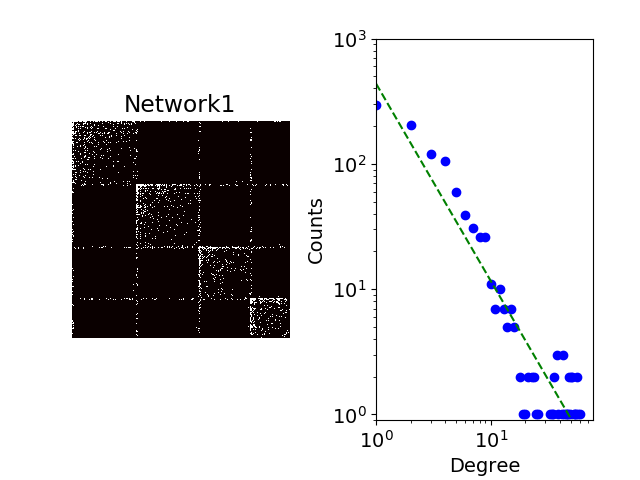
\includegraphics[width=1.1\textwidth]{img/corpus/network1_dd}
        \end{minipage}
        \begin{minipage}{0.4\textwidth}
            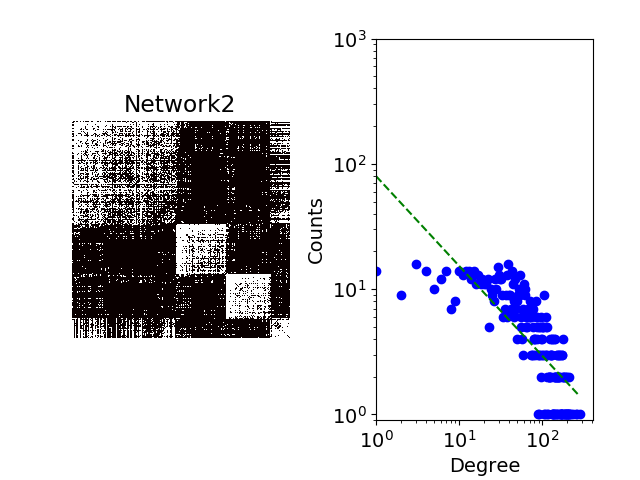
\includegraphics[width=1.1\textwidth]{img/corpus/network2_dd}
        \end{minipage}
        %\vskip\baselineskip
        \begin{minipage}{0.4\textwidth}
            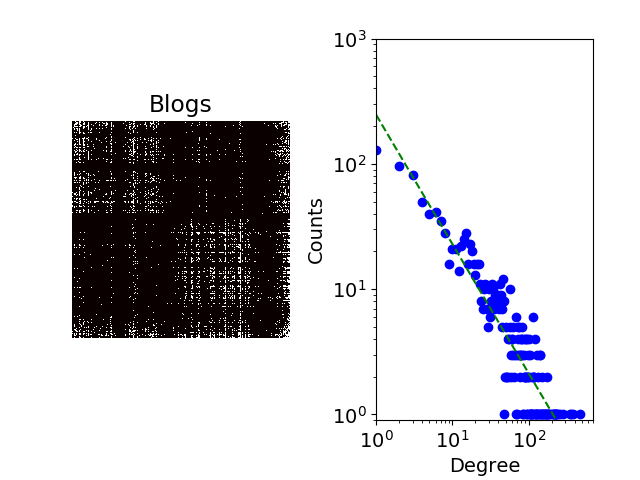
\includegraphics[width=1.1\textwidth]{img/corpus/blogs_dd}
        \end{minipage}
        \begin{minipage}{0.4\textwidth}
            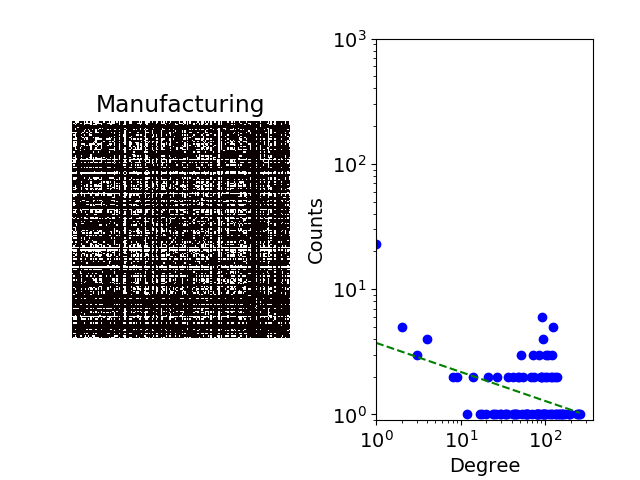
\includegraphics[width=1.1\textwidth]{img/corpus/manufacturing_dd}
        \end{minipage}
	\label{fig:corpuses}
\end{figure}

\begin{figure}[h] {Local degree distributions for the four training datasets. For Network1 and Network2 the classes come from ground-truth. For Blogs and Manufacturing, classes are obtained by Louvain algorithm.} 
        \begin{minipage}{0.4\textwidth}
            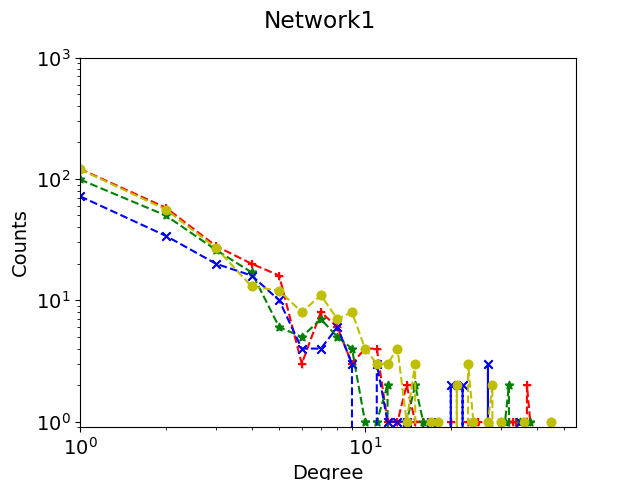
\includegraphics[width=4.22cm,height=3.5cm]{img/corpus/network1_1}
        \end{minipage}
        \begin{minipage}{0.4\textwidth}
            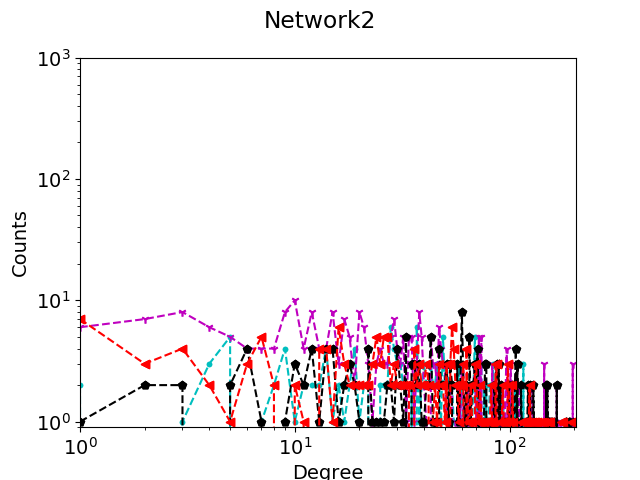
\includegraphics[width=4.22cm,height=3.5cm]{img/corpus/network2_1}
        \end{minipage}
        \vskip\baselineskip
        \begin{minipage}{0.4\textwidth}
            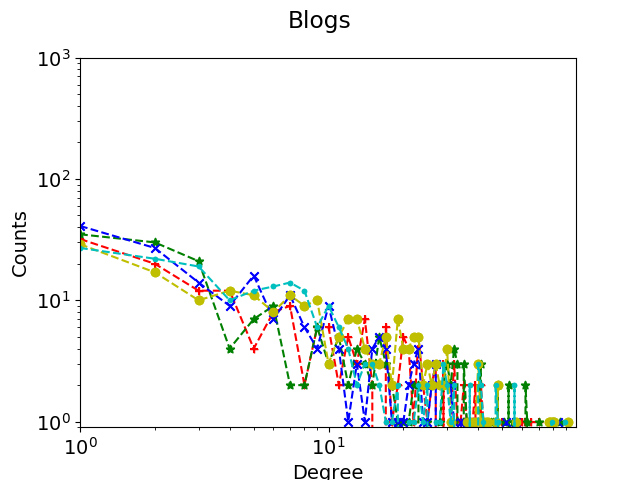
\includegraphics[width=4.22cm,height=3.5cm]{img/corpus/blogs_1}
        \end{minipage}
        \begin{minipage}{0.4\textwidth}
            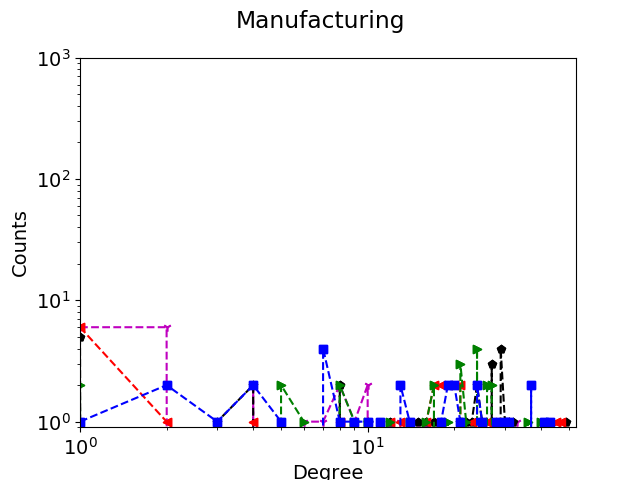
\includegraphics[width=4.22cm,height=3.5cm]{img/corpus/manufacturing_1}
        \end{minipage}
	\label{fig:synt_graph_local}
\end{figure}

For each dataset, we estimate the model parameters through Markov Chain Monte Carlo inference consisting of 200 iterations. For \immsb, the concentration parameters of HDP were optimized  using vague gamma priors $\alpha_0 \sim \text{Gamma}(1,1)$ and $\gamma \sim \text{Gamma}(1,1)$ following \cite{HDP}. The parameters for the matrix weights  $\lambda_0$ and $\lambda_1$ were fixed to 0.1. For \ilfm, the hyperparameter  $\sigma_w$ was fixed to 1 and the IBP hyperparameter $\alpha$ to 0.5 in order to  have comparable number of classes with \immsb. Once the models have been learned, they are used to generate links (or non-links) between the entire set of network nodes. The whole procedure is repeated 10 times and the average values are reported as final results.

\subsection{Homophily}

Figure \ref{fig:homo_mustach} presents boxplots describing the distributions of the natural $s_n(i,j)$ and latent $s_l(i,j)$ similarities computed respectively on linked and non-linked pairs of nodes for \immsb\ (left) and \ilfm\ (right). The results have been aggregated over the four datasets. They confirm that the natural similarity is  higher for pairs of nodes which are linked than for pairs of nodes which are not linked, for both models. For the latent similarity,  there is no difference between the linked and non-linked pairs, indicating that the links are not homophilic. These experimental results are in line with the theoretical results presented in Section~\ref{sec:homophily} that state that both \ilfm\ and \immsb\ are homophilic for  the natural similarity but are not homophilic for the latent similarity.

\begin{figure}[ht]{Natural and latent similarities aggregated over all datasets and computed on linked and non-linked pairs of nodes for \immsb\ (left) and \ilfm\ (right).}
    \begin{subfigure}
       	 \centering
        	 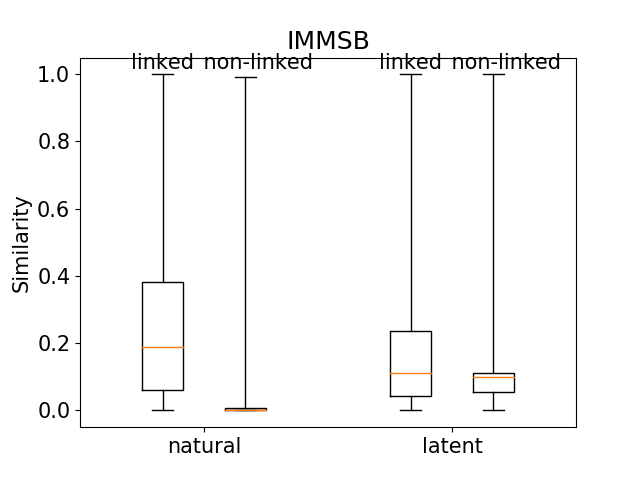
\includegraphics[width=4.22cm,height=3.5cm]{img/corpus/homo_mustach_immsb}
    \end{subfigure}
    \begin{subfigure}
        	 \centering
          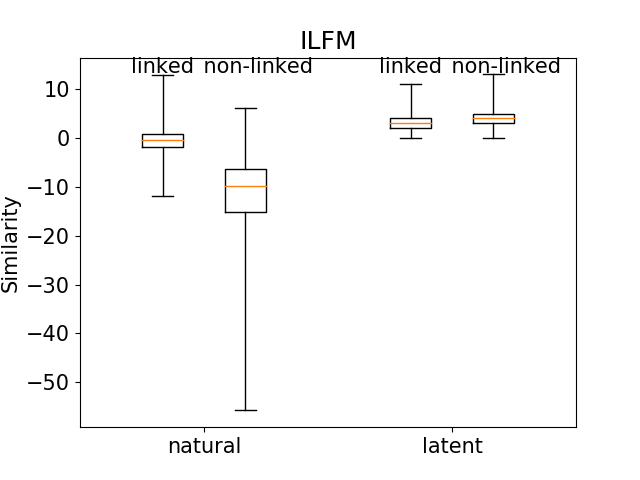
\includegraphics[width=4.22cm,height=3.5cm]{img/corpus/homo_mustach_ilfm}
    \end{subfigure}
    \label{fig:homo_mustach}
\end{figure}

\subsection{Preferential attachment}

Table \ref{table:me_gofit} reports the value of the power-law goodness of fit for \immsb\ and \ilfm\ in the global case (left) and in the local case (right). It appears that for both models, the global preferential attachment is only verified for networks generated from datasets where the property was observed, namely in Network1 with p-value equal to 0.9 for \immsb\ and 1 for \ilfm, and in Blogs with a p-value equal to 1 for both models; the property is not verified in Network2 and in Manufacturing, where p-values are equal to 0. This is in accordance with Proposition 2.1 according to which both \ilfm\ and \immsb\ do not satisfy global preferential attachment. However, these models are able to capture this property if it exists in the training datasets.  Moreover, one can observe that, in the local case, \immsb\ complies with the preferential attachment with $p$-values equal or close to 1 for the four networks, while \ilfm\ obtained low p-values for the networks that were less locally bursty (respectively  0  for Network2 and 0.3 for Manufacturing). In addition, the power-law coefficients $\alpha$ are significantly greater for \immsb\ than for \ilfm, and specially for the bursty networks Network1 and Blogs.

Figure \ref{fig:me_local} illustrates the local preferential attachment for Network1 (top) and Network2 (bottom) estimated with \immsb\ (left) and \ilfm\ (right). The shape of the local degree distributions appears more linear for \immsb\ and with more fluctuations for \ilfm. This illustrates the fact that \ilfm\ does not capture local preferential attachment whereas \immsb\ does, as stated in Proposition 2.2. 


\begin{table}[h]{Preferential attachment measures for training datasets and networks generated with fitted models.}
\begin{tabular}{lrrrr}
  \multirow{2}{*}{\textbf{Training Datasets}}  &
  \multicolumn{2}{c}{Global} & \multicolumn{2}{c}{Local}\\
  \cmidrule(r){2-3} \cmidrule(l){4-5}
  &   $p$-value &   $\alpha$   & $p$-value & $\alpha$   \\
\hline
Network1       & 1 & 2.4 &   1.0 $\pm$ 0.0  &  1.8 $\pm$ 0.03  \\
Network2       & 0 & 1.3 &   0.0 $\pm$ 0.0  &  1.2 $\pm$ 0.01 \\
Blogs          & 1 & 1.5 &   1.0 $\pm$ 0.0  &  1.4 $\pm$ 0.03\\
Manufacturing  & 0 & 1.4 &   0.4 $\pm$ 0.3  &  1.3 $\pm$ 0.05 \\
\hline

  \ \textbf{\immsb} &&&& \\
\hline
Network1       & 0.9 & 1.4 &   1.0 \(\pm\) 0.0   &  3.5 \(\pm\) 0.7 \\
Network2       & 0 & 1.3 &   0.9 \(\pm\) 0.0   &  1.6 \(\pm\) 0.2 \\
Blogs          & 1 & 1.3 &   1.0 \(\pm\) 0.0   &  4.3 \(\pm\) 1.1 \\
Manufacturing  & 0 & 1.2 &   0.9 \(\pm\) 0.01  &  1.6 \(\pm\) 0.1 \\
\hline

  \ \textbf{\ilfm} &&&& \\
\hline
Network1      & 1 & 1.4 &   1.0 \(\pm\) 0.0  &  1.7 \(\pm\) 0.1 \\
Network2      & 0 & 1.2 &   0.0 \(\pm\) 0.0 &  1.2 \(\pm\) 0.0 \\
Blogs         & 1 & 1.3 &   0.9 \(\pm\) 0.2  &  1.5 \(\pm\) 0.1 \\
Manufacturing & 0 & 1.2 &   0.3 \(\pm\) 0.3  &  1.3 \(\pm\) 0.0 \\
\hline
\end{tabular}
\label{table:me_gofit}
\end{table}


\begin{figure}[h]{Local degree distributions for Network1 (top row) and Network2 (bottom row) generated with fitted models \immsb\ (first column) and \ilfm\ (second column).} 
    \begin{minipage}{0.4\textwidth}
        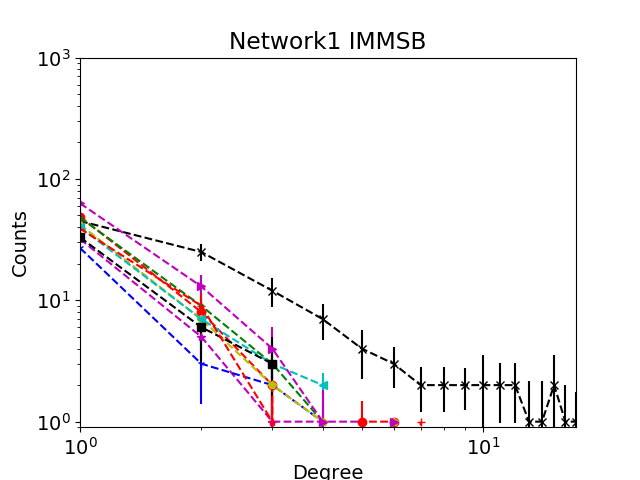
\includegraphics[width=4.22cm,height=3.5cm]{img/corpus/immsb_network1_1}
    \end{minipage}
    \begin{minipage}{0.4\textwidth}
        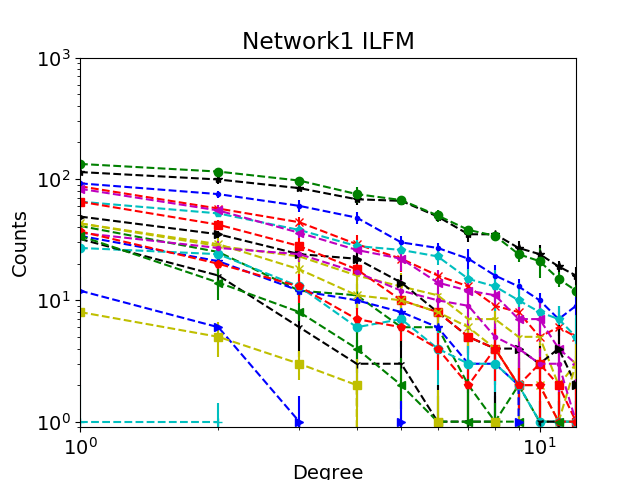
\includegraphics[width=4.22cm,height=3.5cm]{img/corpus/ilfm_network1_1}
    \end{minipage}
    \vskip\baselineskip
    \begin{minipage}{0.4\textwidth}
        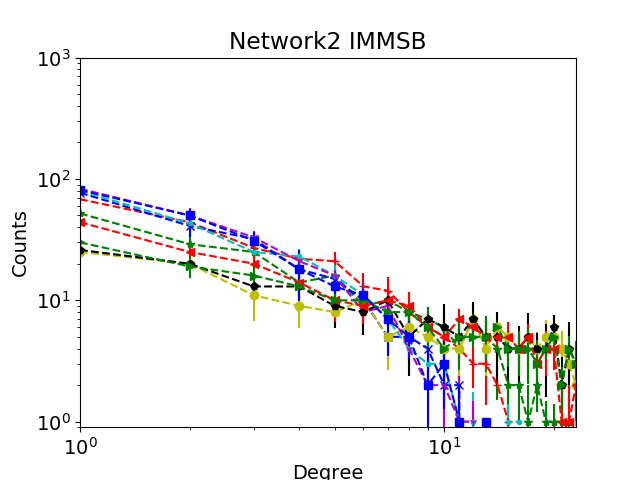
\includegraphics[width=4.22cm,height=3.5cm]{img/corpus/immsb_network2_1}
    \end{minipage}
    \begin{minipage}{0.4\textwidth}
        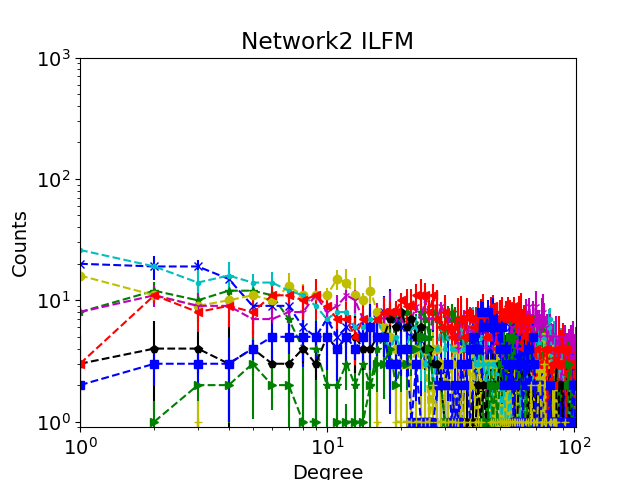
\includegraphics[width=4.22cm,height=3.5cm]{img/corpus/ilfm_network2_1}
    \end{minipage}
\label{fig:me_local}
\end{figure}

\begin{figure}[h] {Top: AUC-ROC curves for Network1 (left) and Network2 (right) with 75 percent of data used for learning. Bottom: Relative performance of \immsb\ and \ilfm\ according to the percentage of data used for testing, the rest being used for learning.} 
    \begin{minipage}{0.4\textwidth}
        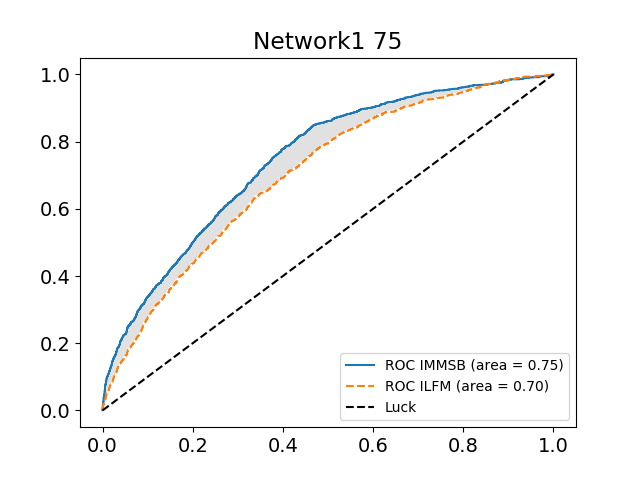
\includegraphics[width=4.22cm,height=3.5cm]{img/corpus/roc_network1_75_f}
    \end{minipage}
    \begin{minipage}{0.4\textwidth}
        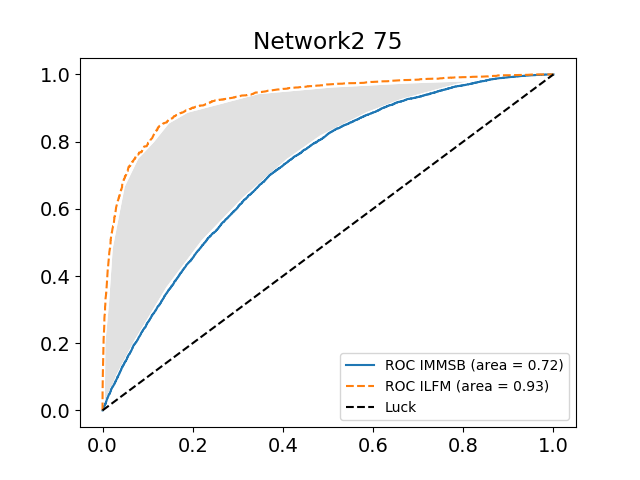
\includegraphics[width=4.22cm,height=3.5cm]{img/corpus/roc_network2_75_f}
    \end{minipage}
    \begin{minipage}{0.5\textwidth}
        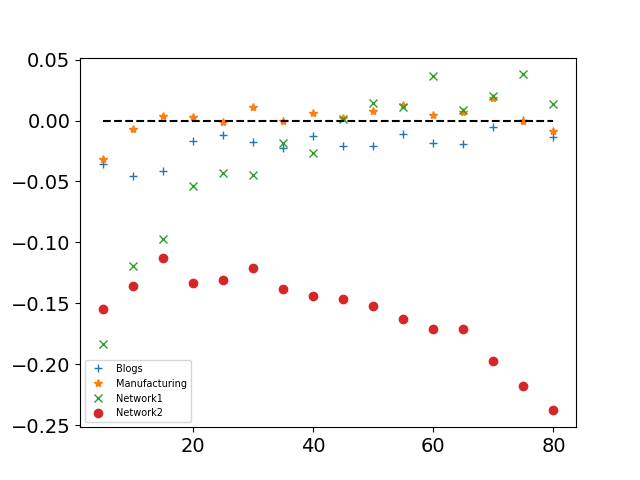
\includegraphics[width=\textwidth]{img/corpus/testset_max_20.png}
    \end{minipage}
\label{fig:auc}
\end{figure}

Lastly, Figure \ref{fig:auc} compares the performance of the models for predicting new links using the Area Under the Curve (AUC) measure as a function of the training set size. In the bottom plot, the y-axis gives the relative performance defined as the difference of the AUC values for \immsb\ and \ilfm\ ($AUC_{\immsb} - AUC_{\ilfm}$) whereas the x-axis indicates the percentage of links randomly removed from the datasets and used as test examples. Hence, the number of training data decreases with the x-axis and a positive value on the y-axis indicates that \immsb\ outperforms \ilfm.  The relative performance corresponds to the difference of the MAX AUC values obtained for both models on the 10 inference experiences. The top plots illustrate a case where 75 percent of the data is used as test set and where \immsb\ dominates \ilfm\ on Network1 (left), and the opposite on Network2 (right).

In general, as shown in the bottom plot, \ilfm\ obtains better performance than \immsb. However, the relative predictive performance of \immsb\  increases  when the quantity of training data decreases on bursty networks, whereas for non-bursty networks the results are the opposite: the performance of \ilfm\ increases when the size of the learning dataset decreases. This is particularly visible for Network2. The results for Manufacturing are less marked, which is certainly due to the small size of this network, making the prediction less challenging.

The above behavior can be explained by the fact that \immsb\ satisfies the local preferential attachment whereas \ilfm\ does not: as links are randomly removed, one is more likely to remove links from large classes than from small ones; a model that enforces local preferential attachment on bursty networks is thus more likely to reconstruct those removed links. This is what is happening on Network1 and Blogs for \immsb. On the contrary, for non-bursty networks, a model enforcing local preferential attachment is penalized.

\section{Conclusion}

We have studied whether stochastic mixed membership models, such as \ilfm\ and \immsb\, can generate new links while satisfying properties frequently verified in real  social networks, namely homophily and preferential attachment. To do so, we have introduced formal definitions of these properties and have analyzed how these models behave according to those definitions. We have shown, in particular, that both models are \textit{homophilic} with the natural similarity that underlies them. Concerning preferential attachment, we have shown that stochastic mixed membership models do not comply with global preferential attachment. The situation is however more contrasted when the property is considered at the local level: \immsb\ enforces local preferential attachment whereas \ilfm\ does not.

These findings have been validated experimentally on two real and two artificial networks that have different degrees of global and local preferential attachment. An important, practical finding of our study is that \immsb, usually considered of lesser "quality" than \ilfm, can indeed yield better results on bursty networks (\textit{i.e.} networks with preferential attachment) when the number of training data is limited.
% This study also paves the way to new models enforcing global preferential attachment through a strict adherence to the definition we have provided.
%
\acknowledgements{Ce travail a été partiellement suporté par la Région Rhône-Alpes.}
 

%\bibliographystyle{unsrt}
\bibliography{./a}

\end{document}
